\documentclass[12pt,a4paper]{article}

% ─── Page Layout ───────────────────────────────────────────────────────────────
\usepackage[a4paper, margin=0.8in, headheight=14pt]{geometry}

% ─── Fonts (XeLaTeX) ───────────────────────────────────────────────────────────
\usepackage{fontspec}
\usepackage{unicode-math}
\setmainfont{TeX Gyre Pagella}
\setmonofont[Scale=0.88]{TeX Gyre Cursor}
\setmathfont{Latin Modern Math}

% ─── Packages ──────────────────────────────────────────────────────────────────
\usepackage{xcolor}
\usepackage{colortbl}
\usepackage{titlesec}
\usepackage{enumitem}
\usepackage{tabularx}
\usepackage{longtable}
\usepackage{booktabs}
\usepackage{array}
\usepackage{amsmath}
\usepackage{tikz}
\usetikzlibrary{shapes.geometric, arrows.meta, positioning, calc, fit, decorations.pathreplacing, patterns}
\usepackage{tcolorbox}
\tcbuselibrary{skins, breakable}
\usepackage{hyperref}
\usepackage{fancyhdr}
\usepackage{graphicx}
\usepackage{microtype}
\hyphenpenalty=10000
\exhyphenpenalty=10000
\sloppy
\usepackage{caption}
\usepackage{setspace}
\usepackage{multirow}
\usepackage{tocloft}

% ─── Q&A helper ────────────────────────────────────────────────────────────────
\newcommand{\Q}[1]{\textbf{#1}\par\noindent\ignorespaces}

% ─── Colour Palette ────────────────────────────────────────────────────────────
\definecolor{myred}{RGB}{196,30,58}
\definecolor{mydark}{RGB}{30,30,50}
\definecolor{mygreen}{RGB}{14,120,80}
\definecolor{myteal}{RGB}{0,130,140}
\definecolor{myamber}{RGB}{180,100,0}
\definecolor{mypurple}{RGB}{100,30,160}
\definecolor{mygray}{RGB}{246,247,249}
\definecolor{mgframe}{RGB}{180,185,200}
\definecolor{watermark}{RGB}{145,150,170}
\definecolor{hdrred}{RGB}{250,232,235}
\definecolor{hdrgreen}{RGB}{220,244,233}
\definecolor{hdrteal}{RGB}{220,242,244}
\definecolor{hdramber}{RGB}{253,242,215}
\definecolor{hdrpurple}{RGB}{238,228,255}
\definecolor{hdrgray}{RGB}{238,240,245}

% ─── Section Formatting ────────────────────────────────────────────────────────
\titleformat{\section}
  {\large\bfseries\color{myred}}{\thesection.}{0.5em}{}
  [\vspace{1pt}{\color{myred}\rule{\linewidth}{0.8pt}}]
\titleformat{\subsection}
  {\normalsize\bfseries\color{myteal}}{\thesubsection}{0.5em}{}
\titlespacing*{\section}{0pt}{18pt}{7pt}
\titlespacing*{\subsection}{0pt}{11pt}{4pt}

% ─── Paragraph ─────────────────────────────────────────────────────────────────
\setlength{\parindent}{0pt}
\setlength{\parskip}{4pt}

% ─── TOC Styling ───────────────────────────────────────────────────────────────
\renewcommand{\cfttoctitlefont}{\large\bfseries\color{myred}}
\renewcommand{\cftaftertoctitle}{\par\noindent{\color{myred}\rule{\linewidth}{0.8pt}}}
\setlength{\cftbeforetoctitleskip}{0pt}
\setlength{\cftaftertoctitleskip}{6pt}
\renewcommand{\cftsecfont}{\normalsize\bfseries\color{mydark}}
\renewcommand{\cftsecpagefont}{\normalsize\bfseries\color{mydark}}
\renewcommand{\cftsecleader}{\cftdotfill{\cftdotsep}}
\setlength{\cftbeforesecskip}{7pt}
\renewcommand{\cftsubsecfont}{\small\color{mydark}}
\renewcommand{\cftsubsecpagefont}{\small\color{mydark}}
\setlength{\cftbeforesubsecskip}{3pt}
\setlength{\cftsubsecindent}{1.4em}

% ─── Table helpers ─────────────────────────────────────────────────────────────
\renewcommand{\arraystretch}{1.45}
\setlength{\tabcolsep}{6pt}
\arrayrulecolor{mydark}
\newcolumntype{B}[1]{>{\small\bfseries\raggedright\arraybackslash}m{#1}}
\newcolumntype{Y}{>{\small\raggedright\arraybackslash}X}
\renewcommand{\tabularxcolumn}[1]{m{#1}}

% ─── Header / Footer ───────────────────────────────────────────────────────────
\pagestyle{fancy}
\fancyhf{}
\fancyhead[L]{\small\color{myred}\textbf{EC403}\;\color{mydark}--- Microprocessor and Microcontroller}
\fancyhead[R]{\small\color{myteal}\textbf{Module 2 Notes}}
\fancyfoot[C]{\small\color{mydark}\thepage}
\fancyfoot[R]{\small\color{watermark}\textit{\copyright\ Biraj Sarkar (CGEC)}}
\renewcommand{\headrulewidth}{0.5pt}
\renewcommand{\footrulewidth}{0.3pt}

% ─── Hyperref ──────────────────────────────────────────────────────────────────
\hypersetup{
  colorlinks=true, linkcolor=myteal, urlcolor=myteal,
  pdfauthor={Biraj Sarkar (CGEC)},
  pdftitle={EC403 --- Module 2 Notes: Peripheral Interfacing and Arithmetic Coprocessors}
}

% ─── tcolorbox styles ──────────────────────────────────────────────────────────
\tcbset{
  tikzbox/.style={
    colback=mygray, colframe=mgframe, boxrule=0.6pt, arc=4pt,
    left=8pt, right=8pt, top=6pt, bottom=6pt,
    colbacktitle=mgframe, coltitle=mydark, fonttitle=\small\bfseries
  },
  defbox/.style={
    colback=hdrgreen, colframe=mygreen, boxrule=0.8pt, arc=4pt,
    left=9pt, right=9pt, top=6pt, bottom=6pt,
    colbacktitle=mygreen, coltitle=white, fonttitle=\small\bfseries
  },
  formulabox/.style={
    colback=hdrteal, colframe=myteal, boxrule=0.8pt, arc=4pt,
    left=9pt, right=9pt, top=7pt, bottom=7pt,
    colbacktitle=myteal, coltitle=white, fonttitle=\small\bfseries
  },
  examplebox/.style={
    colback=hdramber, colframe=myamber, boxrule=0.8pt, arc=4pt,
    left=9pt, right=9pt, top=6pt, bottom=6pt,
    colbacktitle=myamber, coltitle=white, fonttitle=\small\bfseries
  },
  masonbox/.style={
    colback=hdrpurple, colframe=mypurple, boxrule=0.8pt, arc=4pt,
    left=9pt, right=9pt, top=6pt, bottom=6pt,
    colbacktitle=mypurple, coltitle=white, fonttitle=\small\bfseries
  },
  exambox/.style={
    colback=hdrpurple, colframe=mypurple, boxrule=1pt, arc=5pt,
    left=10pt, right=10pt, top=8pt, bottom=8pt,
    colbacktitle=mypurple, coltitle=white, fonttitle=\bfseries,
    breakable, title after break={\textbf{Frequently Asked / Viva Questions (contd.)}}
  }
}
\tcbset{breakable}
\tcbset{after={\par\color{black}}}

% ─── TikZ styles ───────────────────────────────────────────────────────────────
\tikzset{
  block/.style={rectangle, draw=myteal, fill=hdrteal,
    text width=2.4cm, align=center, minimum height=0.95cm,
    font=\small, rounded corners=3pt, line width=0.7pt},
  redblock/.style={rectangle, draw=myred, fill=hdrred,
    text width=2.4cm, align=center, minimum height=0.95cm,
    font=\small, rounded corners=3pt, line width=0.7pt},
  amberblock/.style={rectangle, draw=myamber, fill=hdramber,
    text width=2.4cm, align=center, minimum height=0.95cm,
    font=\small, rounded corners=3pt, line width=0.7pt},
  sumjunc/.style={circle, draw=myamber, fill=hdramber,
    minimum size=0.62cm, font=\small, line width=0.8pt},
  arrow/.style={-Stealth, thick, color=mydark},
  redarrow/.style={-Stealth, thick, color=myred},
  line/.style={thick, color=mydark}
}

\begin{document}

% ─── Title Page ───────────────────────────────────────────────────────────────
\begin{center}
  {\LARGE\bfseries\color{myred} EC403 --- Microprocessor and Microcontroller}\\[5pt]
  {\normalsize\color{mydark} Semester IV \quad$\bullet$\quad 3L:0T:0P \quad$\bullet$\quad 3 Credits}\\[3pt]
  {\normalsize\color{myteal}\textbf{Module 2 Exam Notes: Peripheral Interfacing and Arithmetic Coprocessors}}\\[3pt]
  {\small\color{mydark} CGEC \;$|$\; B.Tech ECE (2023--27) \;$|$\; \textit{Biraj Sarkar}}
\end{center}
\vspace{2pt}
\noindent{\color{myred}\rule{\linewidth}{1.5pt}}
\vspace{2pt}

\hypersetup{linkcolor=mydark}
\tableofcontents
\hypersetup{linkcolor=myteal}
\newpage

\section{Peripheral Interfacing Fundamentals}

\begin{tcolorbox}[defbox, title={Peripheral Interfacing Concepts}]
A \textbf{peripheral interface} connects the central microprocessor to external input/output devices (sensors, keyboards, displays, timers, converters). Because peripherals operate at disparate speeds, signal levels, and data widths, an interfacing IC performs data buffering, address decoding, bus synchronization, and handshaking.
\end{tcolorbox}

\subsection{Memory-Mapped I/O vs. Isolated (I/O-Mapped) I/O}
Microprocessors access peripherals via two distinct addressing topologies:
\par\vspace{6pt}\noindent
\begingroup
\setlength{\extrarowheight}{2.5pt}
\noindent\begin{tabularx}{\linewidth}{|B{3.2cm}|Y|Y|}
\hline
\textbf{Parameter} & \textbf{Isolated (I/O-Mapped) I/O} & \textbf{Memory-Mapped I/O} \\ \hline
Address Space & Separate 8-bit or 16-bit I/O space ($256$ ports in 8085; $64\,\mathrm{KiB}$ in 8086). & Unified memory space; ports share the memory address space ($64\,\mathrm{KiB}$ in 8085; $1\,\mathrm{MiB}$ in 8086). \\ \hline
Access Instructions & Dedicated instructions only: `IN` and `OUT`. & Any memory reference instruction: `MOV`, `LDA`, `STA`, `ADD M`, `CMP M`. \\ \hline
Control Signals & Distinct I/O strobes ($\overline{\mathrm{IOR}}$, $\overline{\mathrm{IOW}}$ or $\mathrm{IO}/\overline{\mathrm{M}}=1$). & Memory strobes ($\overline{\mathrm{MEMR}}$, $\overline{\mathrm{MEMW}}$ or $\mathrm{IO}/\overline{\mathrm{M}}=0$). \\ \hline
Data Registers & Transfers restricted to Accumulator ($A$ or $AX/AL$). & Data transferred to/from any general-purpose CPU register. \\ \hline
Hardware Decoding & Simpler decoding (decodes only 8 address lines $A_0-A_7$). & Full address bus decoding (16 or 20 address lines). \\ \hline
Memory Impact & Preserves full memory capacity for RAM/ROM. & Consumes memory address space; reduces available memory. \\ \hline
\end{tabularx}\par
\endgroup

\section{Intel 8255A Programmable Peripheral Interface (PPI)}

\begin{tcolorbox}[defbox, title={Intel 8255A Architectural Overview}]
The \textbf{Intel 8255A} is a programmable parallel I/O interface in a 40-pin DIP designed to connect peripherals to the system bus. It has 24 programmable I/O lines.
\end{tcolorbox}

\textbf{Port organization.} The 24 I/O lines are arranged in three 8-bit ports.
\begin{itemize}[leftmargin=*]
  \item \textbf{Port A ($PA_7-PA_0$):} 8-bit data input/output latch and buffer.
  \item \textbf{Port B ($PB_7-PB_0$):} 8-bit data input/output latch and buffer.
  \item \textbf{Port C ($PC_7-PC_0$):} Divided into Port C Upper ($PC_7-PC_4$) and Port C Lower ($PC_3-PC_0$); can be used as simple 8-bit I/O or as handshake control signals for Ports A and B.
\end{itemize}


\begin{tcolorbox}[tikzbox, title={Intel 8255A Internal Functional Block Diagram}]
\centering
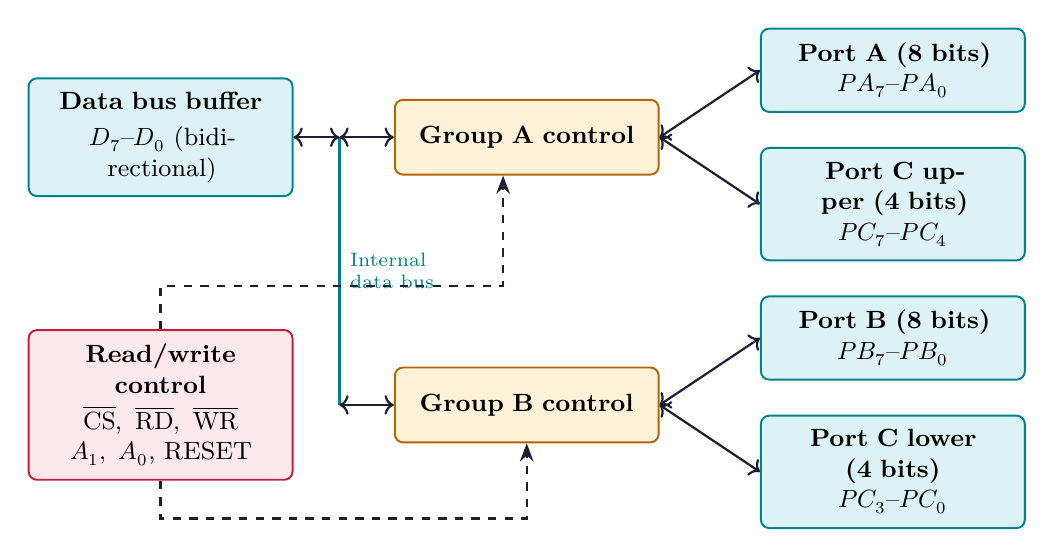
\begin{tikzpicture}[every node/.style={font=\small},
  unit/.style={align=center,text width=3.0cm,inner sep=5pt}]
  \node[block,unit] (buf) at (0,1.7)
    {\textbf{Data bus buffer}\\[2pt] $D_7$--$D_0$ (bidirectional)};
  \node[redblock,unit] (ctrl) at (0,-1.7)
    {\textbf{Read/write control}\\[2pt]
    $\overline{\mathrm{CS}},\ \overline{\mathrm{RD}},\ \overline{\mathrm{WR}}$\\
    $A_1,\ A_0$, RESET};
  \node[amberblock,unit] (a) at (4.65,1.7) {\textbf{Group A control}};
  \node[amberblock,unit] (b) at (4.65,-1.7) {\textbf{Group B control}};
  \node[block,unit] (pa) at (9.3,2.55) {\textbf{Port A (8 bits)}\\ $PA_7$--$PA_0$};
  \node[block,unit] (pcu) at (9.3,0.85) {\textbf{Port C upper (4 bits)}\\ $PC_7$--$PC_4$};
  \node[block,unit] (pb) at (9.3,-0.85) {\textbf{Port B (8 bits)}\\ $PB_7$--$PB_0$};
  \node[block,unit] (pcl) at (9.3,-2.55) {\textbf{Port C lower (4 bits)}\\ $PC_3$--$PC_0$};
  \coordinate (upper) at (2.27,1.7);
  \coordinate (lower) at (2.27,-1.7);
  \draw[very thick,myteal] (upper) -- node[midway,right,font=\scriptsize,align=left]
    {Internal\\data bus} (lower);
  \draw[arrow,<->,thick] (buf.east) -- (upper);
  \draw[arrow,<->,thick] (upper) -- (a.west);
  \draw[arrow,<->,thick] (lower) -- (b.west);
  \draw[arrow,dashed] (ctrl.north) -- ++(0,0.55) -| ([xshift=-3mm]a.south);
  \draw[arrow,dashed] (ctrl.south) -- ++(0,-0.48) -| (b.south);
  \foreach \group/\port in {a/pa,a/pcu,b/pb,b/pcl}
    \draw[arrow,<->,thick] (\group.east) -- (\port.west);
\end{tikzpicture}
\end{tcolorbox}

\subsection{8255A Internal Register Selection}
\par\vspace{6pt}\noindent
\begingroup
\setlength{\extrarowheight}{2.5pt}
\begingroup
\setlength{\LTleft}{0pt}
\setlength{\LTright}{0pt}
\begin{longtable}{|B{1.6cm}|B{1.6cm}|B{1.6cm}|B{1.6cm}|B{1.6cm}|>{\small\raggedright\arraybackslash}m{\dimexpr(\linewidth-1.6cm-1.6cm-1.6cm-1.6cm-1.6cm-12\tabcolsep-7\arrayrulewidth)/1\relax}|}
\hline
$\mathbf{\overline{CS}}$ & $\mathbf{A_1}$ & $\mathbf{A_0}$ & $\mathbf{\overline{RD}}$ & $\mathbf{\overline{WR}}$ & \textbf{Selected 8255A Register / Operation} \\ \hline
\endfirsthead
\hline
$\mathbf{\overline{CS}}$ & $\mathbf{A_1}$ & $\mathbf{A_0}$ & $\mathbf{\overline{RD}}$ & $\mathbf{\overline{WR}}$ & \textbf{Selected 8255A Register / Operation} \\ \hline
\endhead
$0$ & $0$ & $0$ & $0$ & $1$ & Read data from Port A to CPU data bus. \\ \hline
$0$ & $0$ & $0$ & $1$ & $0$ & Write data from CPU data bus to Port A. \\ \hline
$0$ & $0$ & $1$ & $0$ & $1$ & Read data from Port B to CPU data bus. \\ \hline
$0$ & $0$ & $1$ & $1$ & $0$ & Write data from CPU data bus to Port B. \\ \hline
$0$ & $1$ & $0$ & $0$ & $1$ & Read data from Port C to CPU data bus. \\ \hline
$0$ & $1$ & $0$ & $1$ & $0$ & Write data from CPU data bus to Port C. \\ \hline
$0$ & $1$ & $1$ & $1$ & $0$ & Write Control Word to Control Register (Write-only). \\ \hline
$1$ & $\mathrm{X}$ & $\mathrm{X}$ & $\mathrm{X}$ & $\mathrm{X}$ & Chip deselected (tri-state floating data bus). \\ \hline
\end{longtable}
\endgroup\par
\endgroup

\subsection{8255A Control Word Formats}
The 8255 operates in two distinct functional modes determined by bit $D_7$ of the written control word:
\begin{tcolorbox}[formulabox, title={8255A I/O Mode Control Word ($D_7 = 1$)}]
\centering
\begin{tabular}{|c|c|c|c|c|c|c|c|}
\hline
\textbf{$D_7$} & \textbf{$D_6$} & \textbf{$D_5$} & \textbf{$D_4$} & \textbf{$D_3$} & \textbf{$D_2$} & \textbf{$D_1$} & \textbf{$D_0$} \\ \hline
$\mathbf{1}$ & $\mathbf{Mode_A1}$ & $\mathbf{Mode_A0}$ & $\mathbf{PA}$ & $\mathbf{PC_{upper}}$ & $\mathbf{Mode_B}$ & $\mathbf{PB}$ & $\mathbf{PC_{lower}}$ \\ \hline
\end{tabular}
\par\vspace{4pt}\raggedright
\begin{itemize}[leftmargin=*, itemsep=2pt]
  \item \textbf{$D_7 = 1$:} Identifies active Mode Definition (I/O Mode).
  \item \textbf{$D_6, D_5$ (Group A Mode):} $00 = \text{Mode 0}$; $01 = \text{Mode 1}$; $1\mathrm{X} = \text{Mode 2}$.
  \item \textbf{$D_4$ (Port A Direction):} $1 = \text{Input}$; $0 = \text{Output}$.
  \item \textbf{$D_3$ (Port C Upper Direction, $PC_7-PC_4$):} $1 = \text{Input}$; $0 = \text{Output}$.
  \item \textbf{$D_2$ (Group B Mode):} $0 = \text{Mode 0}$; $1 = \text{Mode 1}$.
  \item \textbf{$D_1$ (Port B Direction):} $1 = \text{Input}$; $0 = \text{Output}$.
  \item \textbf{$D_0$ (Port C Lower Direction, $PC_3-PC_0$):} $1 = \text{Input}$; $0 = \text{Output}$.
\end{itemize}
\end{tcolorbox}

\subsection{Operating Modes and Handshake Signals (Mode 1 and Mode 2)}
\begin{enumerate}[leftmargin=*]
  \item \textbf{Mode 0 (Basic Input/Output):} Simple unidirectional I/O without handshaking. Inputs are unlatched; outputs are latched.
  \item \textbf{Mode 1 (Strobed Handshake I/O):} Port A and/or Port B transfer data using dedicated Port C handshake signals:
  \begin{itemize}[leftmargin=*]
    \item \textit{Strobed Input Handshake:}
    \begin{itemize}[leftmargin=*]
      \item $\overline{\mathrm{STB}}$ (Strobe Input): Peripheral pulses low to load byte into 8255 input latch.
      \item $\mathrm{IBF}$ (Input Buffer Full): Output set high by 8255 indicating byte is latched.
      \item $\mathrm{INTR}$ (Interrupt Request): Output high to request CPU service; cleared when CPU reads the port.
    \end{itemize}
    \item \textit{Strobed Output Handshake:}
    \begin{itemize}[leftmargin=*]
      \item $\overline{\mathrm{OBF}}$ (Output Buffer Full): Low when CPU writes data to port; signals peripheral to read.
      \item $\overline{\mathrm{ACK}}$ (Acknowledge Input): Low pulse from peripheral indicating data byte is accepted.
      \item $\mathrm{INTR}$ (Interrupt Request): High when output buffer becomes empty, requesting next byte.
    \end{itemize}
  \end{itemize}
  \item \textbf{Mode 2 (Strobed Bidirectional Bus):} Only Port A operates in Mode 2. Port A becomes an 8-bit bidirectional bus using 5 handshake lines of Port C ($PC_7-PC_3$).
\end{enumerate}

\subsection{8255A Bit Set/Reset (BSR) Mode Control Word}
\begin{tcolorbox}[formulabox, title={8255A Bit Set/Reset (BSR) Mode Control Word ($D_7 = 0$)}]
The BSR mode allows setting or resetting any individual bit of Port C without affecting other Port C pins:
\par\vspace{4pt}
\centering
\begin{tabular}{|c|c|c|c|c|c|c|c|}
\hline
\textbf{$D_7$} & \textbf{$D_6$} & \textbf{$D_5$} & \textbf{$D_4$} & \textbf{$D_3$} & \textbf{$D_2$} & \textbf{$D_1$} & \textbf{$D_0$} \\ \hline
$\mathbf{0}$ & $\mathbf{X}$ & $\mathbf{X}$ & $\mathbf{X}$ & $\mathbf{B_2}$ & $\mathbf{B_1}$ & $\mathbf{B_0}$ & $\mathbf{S/\overline{R}}$ \\ \hline
\end{tabular}
\par\vspace{4pt}\raggedright
\begin{itemize}[leftmargin=*, itemsep=2pt]
  \item \textbf{$D_7 = 0$:} Identifies Bit Set/Reset (BSR) format.
  \item \textbf{$D_6-D_4$:} Don't care ($000_2$ typically).
  \item \textbf{$D_3, D_2, D_1$ (Bit Select):} $000_2 = PC_0$ up to $111_2 = PC_7$.
  \item \textbf{$D_0$ (Set/Reset):} $1 = \text{Set selected bit to 1}$; $0 = \text{Reset selected bit to 0}$.
\end{itemize}
\end{tcolorbox}

\subsection{Keyboard and 7-Segment Display Interfacing with 8255}
\begin{tcolorbox}[examplebox, title={Interfacing a 4x4 Matrix Keyboard to 8255}]
\textbf{Hardware Setup:} Connect Port A ($PA_3-PA_0$) as outputs to 4 keyboard rows; connect Port B ($PB_3-PB_0$) as inputs with pull-up resistors to 4 columns.
\begin{enumerate}[leftmargin=*, itemsep=2pt]
  \item \textbf{Key-Press Detection:} Output all $0$'s on rows ($PA = 00_{\mathrm{H}}$). Read columns from Port B. If all column inputs are $1$, no key is pressed. If any bit is $0$, a key is pressed.
  \item \textbf{Debounce Delay:} Execute a software delay of $20\,\mathrm{ms}$ to eliminate mechanical contact chatter.
  \item \textbf{Key Identification (Row Scan):} Ground one row at a time ($1110_2, 1101_2, 1011_2, 0111_2$) and read Port B columns. The intersecting zero identifies the exact key pressed.
\end{enumerate}
\end{tcolorbox}

\begin{tcolorbox}[examplebox, title={Interfacing Multiplexed 7-Segment Displays to 8255}]
\textbf{Hardware Architecture:}
\begin{itemize}[leftmargin=*, itemsep=2pt]
  \item \textbf{Segment Data Bus (Port A):} Connect $PA_7-PA_0$ through current-limiting resistors ($330\,\Omega$) to display segments ($dp, g, f, e, d, c, b, a$).
  \item \textbf{Digit Multiplexing Control (Port B):} Connect $PB_3-PB_0$ to switching transistor drivers (BC547) controlling common cathodes of 4 display digits.
\end{itemize}
\par\vspace{3pt}
\textbf{Common-Cathode 7-Segment Hex Code Lookup Table:}
\par\vspace{2pt}
\begingroup
\setlength{\extrarowheight}{2pt}
\noindent\begin{tabularx}{\linewidth}{|B{2.2cm}|B{1.6cm}|B{2.2cm}|B{1.6cm}|B{2.2cm}|Y|}
\hline
\textbf{Digit} & \textbf{Hex Code} & \textbf{Digit} & \textbf{Hex Code} & \textbf{Digit} & \textbf{Hex Code} \\ \hline
0 & \texttt{3FH} & 4 & \texttt{66H} & 8 & \texttt{7FH} \\ \hline
1 & \texttt{06H} & 5 & \texttt{6DH} & 9 & \texttt{6FH} \\ \hline
2 & \texttt{5BH} & 6 & \texttt{7DH} & A & \texttt{77H} \\ \hline
3 & \texttt{4FH} & 7 & \texttt{07H} & E & \texttt{79H} \\ \hline
\end{tabularx}\par
\endgroup
\par\vspace{3pt}
\textbf{Dynamic Scanning:} Digits are refreshed sequentially at $\sim 2\text{--}5\,\mathrm{ms}$ per digit ($>50\,\mathrm{Hz}$ total rate), providing steady, flicker-free illumination via \textbf{Persistence of Vision (POV)}.
\end{tcolorbox}

\section{Intel 8253 / 8254 Programmable Interval Timer (PIT)}

\begin{tcolorbox}[defbox, title={Intel 8253/8254 Architectural Overview}]
The \textbf{Intel 8253/8254} is a programmable counter/timer designed to generate accurate hardware delays, square waves, and event counts. It contains three independent 16-bit counters (Counter 0, 1, 2) that operate in binary or BCD counting down from a loaded count value.
\end{tcolorbox}

\subsection{Control Word Register Format}
\begin{tcolorbox}[formulabox, title={8253/8254 Control Word Format}]
\centering
\begin{tabular}{|c|c|c|c|c|c|c|c|}
\hline
\textbf{$D_7$} & \textbf{$D_6$} & \textbf{$D_5$} & \textbf{$D_4$} & \textbf{$D_3$} & \textbf{$D_2$} & \textbf{$D_1$} & \textbf{$D_0$} \\ \hline
$\mathbf{SC_1}$ & $\mathbf{SC_0}$ & $\mathbf{RW_1}$ & $\mathbf{RW_0}$ & $\mathbf{M_2}$ & $\mathbf{M_1}$ & $\mathbf{M_0}$ & $\mathbf{BCD}$ \\ \hline
\end{tabular}
\par\vspace{4pt}\raggedright
\begin{itemize}[leftmargin=*, itemsep=2pt]
  \item \textbf{$SC_1, SC_0$ (Select Counter):} $00 = \text{Counter 0}$; $01 = \text{Counter 1}$; $10 = \text{Counter 2}$; $11 = \text{Read-Back Command (8254)}$.
  \item \textbf{$RW_1, RW_0$ (Read/Write):} $00 = \text{Counter Latch}$; $01 = \text{Read/Write LSB only}$; $10 = \text{Read/Write MSB only}$; $11 = \text{Read/Write LSB first, then MSB}$.
  \item \textbf{$M_2, M_1, M_0$ (Operating Mode):} $000 = \text{Mode 0}$; $001 = \text{Mode 1}$; $\mathrm{X}10 = \text{Mode 2}$; $\mathrm{X}11 = \text{Mode 3}$; $100 = \text{Mode 4}$; $101 = \text{Mode 5}$.
  \item \textbf{BCD:} $0 = \text{16-bit Binary Counter (0 to 65535)}$; $1 = \text{4-decade BCD Counter (0 to 9999)}$.
\end{itemize}
\end{tcolorbox}

\subsection{The Six Operating Modes of 8253/8254}
\par\vspace{6pt}\noindent
\begingroup
\setlength{\extrarowheight}{2.5pt}
\begingroup
\setlength{\LTleft}{0pt}
\setlength{\LTright}{0pt}
\begin{longtable}{|B{1.8cm}|B{3.2cm}|>{\small\raggedright\arraybackslash}m{\dimexpr(\linewidth-1.8cm-3.2cm-6\tabcolsep-4\arrayrulewidth)/1\relax}|}
\hline
\textbf{Mode} & \textbf{Mode Designation} & \textbf{Operating Waveform Behavior and Applications} \\ \hline
\endfirsthead
\hline
\textbf{Mode} & \textbf{Mode Designation} & \textbf{Operating Waveform Behavior and Applications} \\ \hline
\endhead
Mode 0 & Interrupt on Terminal Count & Output low upon writing control word; stays low while counting down. Goes high when counter reaches zero and stays high until reloaded. \\ \hline
Mode 1 & Hardware Retriggerable One-Shot & Output goes low on rising edge of GATE; stays low for $N$ clock cycles, then returns high. A new GATE trigger restarts the pulse. \\ \hline
Mode 2 & Rate Generator (Divide-by-N) & Output remains high for $N-1$ clock periods, pulses low for exactly 1 clock period, and automatically reloads $N$ (Periodic pulse train). \\ \hline
Mode 3 & Square Wave Generator & Output is high for $\lceil N/2 \rceil$ counts and low for $\lfloor N/2 \rfloor$ counts ($50\%$ duty cycle). Used for baud-rate generation and clocks. \\ \hline
Mode 4 & Software Triggered Strobe & Output is high while counting; pulses low for 1 clock cycle upon reaching terminal count. Counting is started by loading the count. \\ \hline
Mode 5 & Hardware Triggered Strobe & Counting starts on rising edge of GATE; output pulses low for 1 clock period upon terminal count. Retriggerable by GATE. \\ \hline
\end{longtable}
\endgroup\par
\endgroup

\subsection{Key Differences: Intel 8253 vs. Intel 8254}
\begin{itemize}[leftmargin=*]
  \item \textbf{Maximum Operating Clock Frequency:} 8253 has a maximum clock limit of $2.6\,\mathrm{MHz}$; 8254 operates up to $8\,\mathrm{MHz}$ (8254-2 up to $10\,\mathrm{MHz}$).
  \item \textbf{Read-Back Command:} Exclusive to the 8254 ($SC_1SC_0 = 11_2$). Allows reading the count, current mode, and null count status of multiple counters simultaneously.
  \item \textbf{Status Latching:} 8254 can latch counter status alongside count data; 8253 can only latch count values.
\end{itemize}

\section{Intel 8251A USART (Serial Communication Interface)}

\begin{tcolorbox}[defbox, title={Intel 8251A USART Overview}]
The \textbf{Intel 8251A USART} (Universal Synchronous/Asynchronous Receiver/Transmitter) is a programmable communications chip that converts parallel data from the CPU into a serial bit stream for transmission, and converts received serial streams back into parallel bytes.
\end{tcolorbox}

\subsection{Asynchronous Framing and Baud Rate Generation}
\begin{itemize}[leftmargin=*]
  \item \textbf{Asynchronous Frame Structure:} Idle Mark ($1$), Start Bit ($0$), $5$ to $8$ Data Bits (LSB first), Optional Parity Bit (Odd or Even), and $1$, $1.5$, or $2$ Stop Bits ($1$).
  \item \textbf{Baud Rate Calculation:}
  \[
  \mathbf{\mathrm{Baud\ Rate}} = \frac{f_{\mathrm{TxC}}}{\text{Baud Factor}} = \frac{f_{\mathrm{CLK}}}{\text{Prescaler} \times \text{Count}}
  \]
  where Baud Factor $\in \{1\times, 16\times, 64\times\}$ configured in the Mode Instruction Word.
  \item \textbf{RS-232C Standard and MAX232 Level Converter:}
  RS-232C defines logic $1$ (Mark) as $-3\,\mathrm{V}$ to $-15\,\mathrm{V}$, and logic $0$ (Space) as $+3\,\mathrm{V}$ to $+15\,\mathrm{V}$. A \textbf{MAX232} IC uses internal charge-pump capacitors ($0.1\,\mu\mathrm{F}$) to convert TTL $0\,\mathrm{V}/+5\,\mathrm{V}$ levels to true RS-232C bipolar voltages.
\end{itemize}

\begin{tcolorbox}[formulabox, title={8251A Mode Instruction Word (Asynchronous)}]
\centering
\begin{tabular}{|c|c|c|c|c|c|c|c|}
\hline
\textbf{$D_7$} & \textbf{$D_6$} & \textbf{$D_5$} & \textbf{$D_4$} & \textbf{$D_3$} & \textbf{$D_2$} & \textbf{$D_1$} & \textbf{$D_0$} \\ \hline
$\mathbf{S_2}$ & $\mathbf{S_1}$ & $\mathbf{EP}$ & $\mathbf{PEN}$ & $\mathbf{L_2}$ & $\mathbf{L_1}$ & $\mathbf{B_2}$ & $\mathbf{B_1}$ \\ \hline
\end{tabular}
\par\vspace{3pt}\raggedright
\begin{itemize}[leftmargin=*, itemsep=1pt]
  \item \textbf{$B_2, B_1$ (Baud Factor):} $01 = 1\times$; $10 = 16\times$; $11 = 64\times$ ($00 = \text{Synchronous Mode}$).
  \item \textbf{$L_2, L_1$ (Character Length):} $00 = 5\text{ bits}$; $01 = 6\text{ bits}$; $10 = 7\text{ bits}$; $11 = 8\text{ bits}$.
  \item \textbf{PEN, EP (Parity):} $\mathrm{PEN}=1$ enables parity; $\mathrm{EP}=1$ selects Even parity ($0 = \text{Odd}$).
  \item \textbf{$S_2, S_1$ (Stop Bits):} $01 = 1\text{ stop bit}$; $10 = 1.5\text{ stop bits}$; $11 = 2\text{ stop bits}$.
\end{itemize}
\end{tcolorbox}

\section{Analog-to-Digital and Digital-to-Analog Interfacing}

\subsection{ADC 0808 / 0809 Successive Approximation Interfacing}
\begin{tcolorbox}[defbox, title={ADC 0808 / 0809 Specifications}]
The \textbf{ADC 0808} is an 8-bit analog-to-digital converter featuring an on-chip 8-channel multiplexer, successive approximation conversion, and tri-state output latches. It accepts an input voltage range of $0\,\mathrm{V}$ to $+5\,\mathrm{V}$ and provides a step resolution of $\Delta V = \frac{V_{ref}}{2^8} = \frac{5\,\mathrm{V}}{256} = 19.53\,\mathrm{mV}$.
\end{tcolorbox}

\begin{itemize}[leftmargin=*]
  \item \textbf{Control Pins and Handshake Sequence:}
  \begin{enumerate}[leftmargin=*]
    \item \textbf{Channel Select ($A, B, C$) \& ALE:} Apply 3-bit channel address ($000_2$ for $\mathrm{IN}_0$ to $111_2$ for $\mathrm{IN}_7$) and pulse Address Latch Enable ($\mathrm{ALE}$) high to select channel.
    \item \textbf{Start of Conversion (START / SOC):} Pulse $\mathrm{START}$ high ($\ge 100\,\mathrm{ns}$) to reset internal registers and commence conversion.
    \item \textbf{End of Conversion (EOC):} Goes low during conversion; rises high when conversion finishes.
    \item \textbf{Output Enable (OE):} Driven high by CPU to place the 8-bit digital output on the data bus.
  \end{enumerate}
  \item \textbf{Conversion Time:} $T_C = 64 \times T_{CLK} = 64 \times \frac{1}{640\,\mathrm{kHz}} = 100\,\mu\mathrm{s}$.
\end{itemize}

\begin{tcolorbox}[tikzbox, title={ADC 0808 Interfacing with Microprocessor Bus}]
\centering
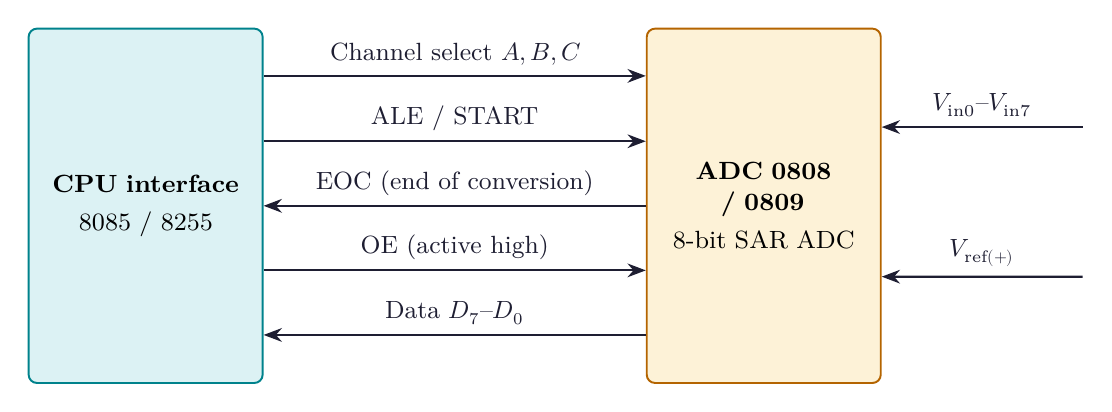
\begin{tikzpicture}[every node/.style={font=\small},
  unit/.style={align=center,text width=2.55cm,inner sep=6pt,minimum height=4.5cm}]
  \node[block,unit] (cpu) at (0,0) {\textbf{CPU interface}\\[3pt] 8085 / 8255};
  \node[amberblock,unit] (adc) at (7.85,0) {\textbf{ADC 0808 / 0809}\\[3pt] 8-bit SAR ADC};
  \foreach \level/\label in {1.65/{Channel select $A,B,C$},
    0.82/{ALE / START},-0.82/{OE (active high)}} {
    \draw[arrow,thick] ([yshift=\level cm]cpu.east) --
      node[above] {\label} ([yshift=\level cm]adc.west);
  }
  \foreach \level/\label in {0/{EOC (end of conversion)},-1.64/{Data $D_7$--$D_0$}} {
    \draw[arrow,thick] ([yshift=\level cm]adc.west) --
      node[above] {\label} ([yshift=\level cm]cpu.east);
  }
  \draw[arrow,thick] (11.9,1.0) -- node[above] {$V_{\mathrm{in0}}$--$V_{\mathrm{in7}}$}
    ([yshift=1cm]adc.east);
  \draw[arrow,thick] (11.9,-0.9) -- node[above] {$V_{\mathrm{ref}(+)}$}
    ([yshift=-0.9cm]adc.east);
\end{tikzpicture}
\end{tcolorbox}

\subsection{DAC 0808 Digital-to-Analog Interfacing}
\begin{tcolorbox}[defbox, title={DAC 0808 Specifications}]
The \textbf{DAC 0808} is an 8-bit monolithic multiplying D/A converter using an R-2R ladder network. It generates an output current proportional to the digital input byte:
\[
\mathbf{I_{\mathrm{out}}} = I_{\mathrm{ref}} \left( \frac{D_7}{2} + \frac{D_6}{4} + \frac{D_5}{8} + \cdots + \frac{D_0}{256} \right) = \frac{V_{\mathrm{ref}}}{R_{\mathrm{ref}}} \left( \frac{\text{Digital Code}}{256} \right)
\]
To obtain an analog voltage, $I_{\mathrm{out}}$ is fed into the inverting summing node of an external Op-Amp (e.g., OP-07 / LM741) with feedback resistor $R_f$:
\[
\mathbf{V_{\mathrm{out}}} = -I_{\mathrm{out}} R_f = -V_{\mathrm{ref}} \left(\frac{R_f}{R_{\mathrm{ref}}}\right) \left( \frac{\text{Digital Code}}{256} \right)
\]
\end{tcolorbox}

\begin{tcolorbox}[examplebox, title={Generating a Triangular Waveform with DAC 0808}]
\textbf{8085 Assembly Code:} Connect DAC input to 8255 Port A (\texttt{80H}).
\begin{verbatim}
        MVI  A, 80H     ; Configure 8255 Port A as Output in Mode 0
        OUT  83H        ; Write to Control Register
LOOP1:  MVI  A, 00H     ; Start at 00H
UP:     OUT  80H        ; Output to DAC
        INR  A          ; Step upward
        JNZ  UP         ; Loop until overflow (00H)
DOWN:   DCR  A          ; Step downward
        OUT  80H        ; Output to DAC
        JNZ  DOWN       ; Loop until 00H reached
        JMP  LOOP1      ; Repeat triangular wave continuously
\end{verbatim}
\end{tcolorbox}

\begin{tcolorbox}[tikzbox, title={DAC 0808 Interfacing with Op-Amp Current-to-Voltage Converter}]
\centering
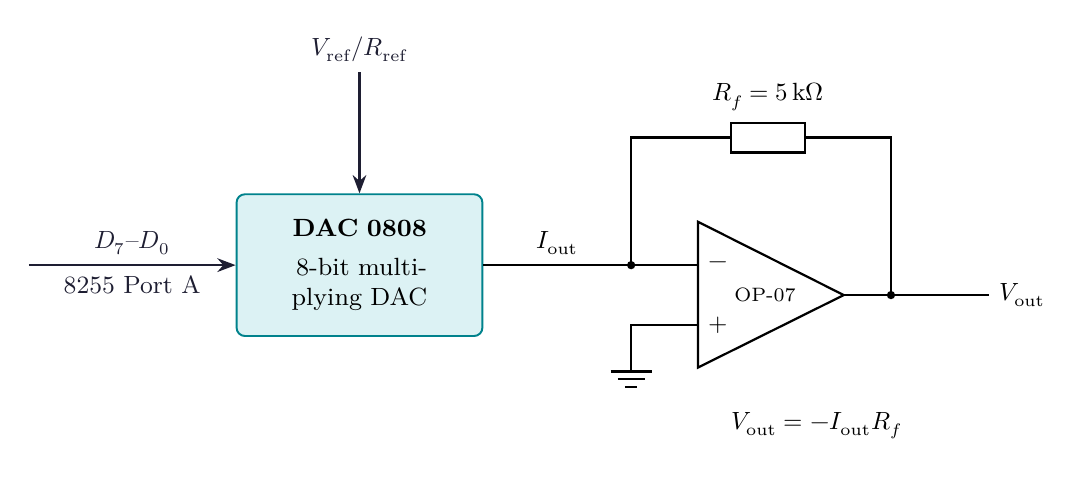
\begin{tikzpicture}[every node/.style={font=\small}]
  \node[block,align=center,text width=2.7cm,inner sep=6pt,minimum height=1.8cm]
    (dac) at (0,0) {\textbf{DAC 0808}\\[3pt] 8-bit multiplying DAC};
  \draw[arrow,thick] (-4.2,0) -- node[above] {$D_7$--$D_0$}
    node[below] {8255 Port A} (dac.west);
  \draw[arrow,thick] (0,2.45) node[above] {$V_{\mathrm{ref}}/R_{\mathrm{ref}}$} -- (dac.north);

  \draw[thick] (4.3,0.55) -- (4.3,-1.30) -- (6.15,-0.38) -- cycle;
  \node at (4.55,0) {$-$};
  \node at (4.55,-0.76) {$+$};
  \node[font=\scriptsize] at (5.15,-0.38) {OP-07};
  \coordinate (sum) at (3.45,0);
  \coordinate (output) at (6.75,-0.38);
  \draw[thick] (dac.east) -- node[above] {$I_{\mathrm{out}}$} (sum) -- (4.3,0);
  \draw[thick] (4.3,-0.76) -- (3.45,-0.76) -- (3.45,-1.35);
  \draw[thick] (3.19,-1.35) -- (3.71,-1.35)
    (3.28,-1.45) -- (3.62,-1.45) (3.37,-1.55) -- (3.53,-1.55);
  \draw[thick] (6.15,-0.38) -- (output) -- (8.0,-0.38)
    node[right] {$V_{\mathrm{out}}$};

  \draw[thick] (sum) -- (3.45,1.62) -- (4.72,1.62);
  \draw[thick] (4.72,1.43) rectangle (5.66,1.81);
  \node[above] at (5.19,1.84) {$R_f=5\,\mathrm{k}\Omega$};
  \draw[thick] (5.66,1.62) -| (output);
  \fill (sum) circle[radius=1.5pt] (output) circle[radius=1.5pt];
  \node[below] at (5.8,-1.75) {$V_{\mathrm{out}}=-I_{\mathrm{out}}R_f$};
\end{tikzpicture}
\end{tcolorbox}

\section{Intel 8087 Numeric Coprocessor}

\begin{tcolorbox}[defbox, title={Intel 8087 Math Coprocessor Overview}]
The \textbf{Intel 8087 Numeric Data Processor (NDP)} is an arithmetic coprocessor that operates closely coupled with the 8086 in Maximum Mode. It accelerates floating-point arithmetic, transcendental, logarithmic, and trigonometric calculations by a factor of $50\times$ to $100\times$ compared to software routines.
\end{tcolorbox}

\begin{itemize}[leftmargin=*]
  \item \textbf{Internal Architecture:}
  \begin{itemize}[leftmargin=*]
    \item \textbf{Control Unit (CU):} Monitors the 8086 bus instruction stream. Decodes `ESC` (Escape) opcodes ($D8_{\mathrm{H}}-DF_{\mathrm{H}}$) and maintains an identical instruction queue.
    \item \textbf{Numeric Execution Unit (NEU):} Executes mathematical operations using an 8-deep register stack ($ST(0)$ to $ST(7)$), with each register having an 80-bit extended-precision width.
  \end{itemize}
  \item \textbf{IEEE 754 Floating-Point Formats:}
  \begin{itemize}[leftmargin=*]
    \item \textbf{Single Precision (32-bit):} 1 sign bit ($s$), 8-bit biased exponent ($e$, bias $= 127$), 23-bit mantissa ($m$).
    \item \textbf{Double Precision (64-bit):} 1 sign bit ($s$), 11-bit biased exponent ($e$, bias $= 1023$), 52-bit mantissa ($m$).
    \item \textbf{Extended Precision (80-bit):} 1 sign bit ($s$), 15-bit biased exponent ($e$, bias $= 16383$), 64-bit mantissa ($m$).
  \end{itemize}
  \item \textbf{8086--8087 Maximum Mode Interfacing:}
  The 8086 and 8087 share the multiplexed address/data bus, status lines, and clock. When the 8087 is busy computing, it asserts its $\mathrm{BUSY}$ output pin. The 8086 connects its $\overline{\mathrm{TEST}}$ input pin to the 8087 $\mathrm{BUSY}$ pin. The 8086 executes a `WAIT` instruction before accessing shared results, pausing until $\overline{\mathrm{TEST}}$ goes low (8087 idle).
\end{itemize}

\begin{tcolorbox}[formulabox, title={8087 Status Word Format and Condition Codes}]
\par\vspace{2pt}
\begingroup
\setlength{\extrarowheight}{2pt}
\noindent\begin{tabularx}{\linewidth}{|B{2.4cm}|B{2.0cm}|Y|}
\hline
\textbf{Status Bit} & \textbf{Bit Field} & \textbf{Architectural Significance} \\ \hline
$B$ & Bit 15 & Coprocessor Busy flag ($1 = \text{executing instruction}$; $0 = \text{idle}$). \\ \hline
$C_3, C_2, C_1, C_0$ & Bits 14, 10, 9, 8 & Condition Code bits reflecting results of comparisons (`FCOM`, `FTST`). \\ \hline
$\mathrm{TOP}$ & Bits 13--11 & Stack Top pointer ($000_2$ to $111_2$) pointing to active $ST(0)$ register. \\ \hline
$\mathrm{ES}$ & Bit 7 & Error Summary flag; set if any unmasked numerical exception occurs. \\ \hline
Exceptions & Bits 5--0 & Flags: Precision, Underflow, Overflow, Zero-divide, Denormal, Invalid. \\ \hline
\end{tabularx}\par
\endgroup
\end{tcolorbox}

\section{System-Level Interfacing Design}

\begin{tcolorbox}[examplebox, title={Complete 8085 Microprocessor System Interfacing Design}, breakable]
\textbf{System Specification:} Design an 8085-based microcomputer system with:
\begin{itemize}[leftmargin=*]
  \item $8\,\mathrm{KiB}$ EPROM (2764) starting at \texttt{0000H}.
  \item $8\,\mathrm{KiB}$ SRAM (6264) starting at \texttt{8000H}.
  \item $8255\,\mathrm{PPI}$ for parallel I/O mapped to ports \texttt{20H}--\texttt{23H}.
  \item $8253\,\mathrm{PIT}$ for timing mapped to ports \texttt{40H}--\texttt{43H}.
\end{itemize}
\par\vspace{4pt}
\textbf{Address Decoding Map (74LS138):}
\par\vspace{4pt}
\begingroup
\setlength{\extrarowheight}{2.5pt}
\noindent\begin{tabularx}{\linewidth}{|B{2.2cm}|B{3.2cm}|B{2.0cm}|B{2.4cm}|Y|}
\hline
\textbf{Device} & \textbf{Address Range} & $\mathbf{IO/\overline{M}}$ & $\mathbf{A_{15}A_{14}A_{13}}$ & \textbf{Chip Select Decoding} \\ \hline
EPROM (2764) & \texttt{0000H}--\texttt{1FFFH} & $0$ & $000_2$ & $\overline{Y}_0$ of Memory Decoder ($\overline{\mathrm{CS}}_1$) \\ \hline
SRAM (6264) & \texttt{8000H}--\texttt{9FFFH} & $0$ & $100_2$ & $\overline{Y}_4$ of Memory Decoder ($\overline{\mathrm{CS}}_2$) \\ \hline
8255 PPI & \texttt{20H}--\texttt{23H} & $1$ & $001_2$ ($A_7A_6A_5$) & $\overline{Y}_1$ of I/O Decoder ($\overline{\mathrm{CS}}_{PPI}$) \\ \hline
8253 PIT & \texttt{40H}--\texttt{43H} & $1$ & $010_2$ ($A_7A_6A_5$) & $\overline{Y}_2$ of I/O Decoder ($\overline{\mathrm{CS}}_{PIT}$) \\ \hline
\end{tabularx}\par
\endgroup
\par\vspace{6pt}
\textbf{System Interconnection Architecture:}
\begin{enumerate}[leftmargin=*]
  \item Demultiplex $AD_0-AD_7$ using a 74LS373 latch with $\mathrm{ALE}$ strobe to generate stable $A_0-A_7$.
  \item Buffer $D_0-D_7$ using a 74LS245 bidirectional transceiver driven by $\overline{\mathrm{RD}}$ for direction.
  \item Memory Decoder (74LS138): Connect $A_{15}, A_{14}, A_{13}$ to inputs $C, B, A$. Set $E_1 = \mathrm{GND}$, $E_2 = \mathrm{IO}/\overline{\mathrm{M}}$ (active low), $E_3 = +5\,\mathrm{V}$. Connect $\overline{Y}_0 \to \overline{\mathrm{CS}}$ of 2764; connect $\overline{Y}_4 \to \overline{\mathrm{CS}}$ of 6264.
  \item Generate $\overline{\mathrm{MEMR}} = \mathrm{OR}(IO/\overline{\mathrm{M}}, \overline{\mathrm{RD}})$ and $\overline{\mathrm{MEMW}} = \mathrm{OR}(IO/\overline{\mathrm{M}}, \overline{\mathrm{WR}})$.
  \item Connect $\overline{\mathrm{MEMR}}$ to $\overline{\mathrm{OE}}$ of EPROM and SRAM; connect $\overline{\mathrm{MEMW}}$ to $\overline{\mathrm{WE}}$ of SRAM.
\end{enumerate}
\end{tcolorbox}

\begin{tcolorbox}[tikzbox, title={Complete 8085 System Interfacing Block Diagram}]
\centering
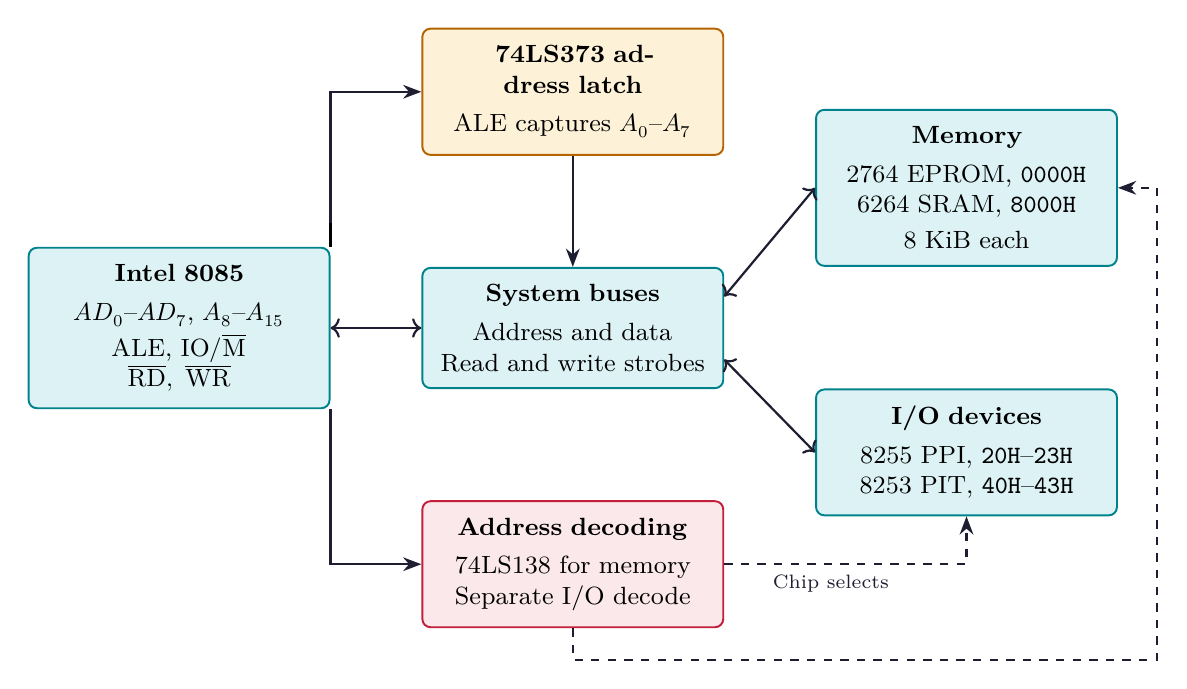
\begin{tikzpicture}[every node/.style={font=\small},
  unit/.style={align=center,text width=3.4cm,inner sep=6pt}]
  \node[block,unit] (cpu) at (0,0)
    {\textbf{Intel 8085}\\[3pt] $AD_0$--$AD_7$, $A_8$--$A_{15}$\\[2pt]
    ALE, $\mathrm{IO}/\overline{\mathrm{M}}$\\
    $\overline{\mathrm{RD}},\ \overline{\mathrm{WR}}$};
  \node[amberblock,unit] (latch) at (5.0,3.0)
    {\textbf{74LS373 address latch}\\[3pt] ALE captures $A_0$--$A_7$};
  \node[block,unit] (bus) at (5.0,0)
    {\textbf{System buses}\\[3pt] Address and data\\
    Read and write strobes};
  \node[redblock,unit] (decode) at (5.0,-3.0)
    {\textbf{Address decoding}\\[3pt] 74LS138 for memory\\ Separate I/O decode};
  \node[block,unit] (mem) at (10,1.78)
    {\textbf{Memory}\\[3pt] 2764 EPROM, \texttt{0000H}\\
    6264 SRAM, \texttt{8000H}\\[2pt] 8 KiB each};
  \node[block,unit] (io) at (10,-1.58)
    {\textbf{I/O devices}\\[3pt] 8255 PPI, \texttt{20H}--\texttt{23H}\\
    8253 PIT, \texttt{40H}--\texttt{43H}};
  \draw[arrow,thick] ([yshift=3mm]cpu.north east) |- (latch.west);
  \draw[thick] (cpu.north east) -- ([yshift=3mm]cpu.north east);
  \draw[arrow,<->,thick] (cpu.east) -- (bus.west);
  \draw[arrow,thick] (cpu.south east) |- (decode.west);
  \draw[arrow,thick] (latch.south) -- (bus.north);
  \draw[arrow,<->,thick] ([yshift=4mm]bus.east) -- (mem.west);
  \draw[arrow,<->,thick] ([yshift=-4mm]bus.east) -- (io.west);
  \draw[arrow,thick,dashed] (decode.east) -|
    node[pos=0.22,below,font=\scriptsize] {Chip selects} (io.south);
  \draw[arrow,thick,dashed] (decode.south) -- ++(0,-0.40) -|
    ([xshift=5mm]mem.east) -- (mem.east);
\end{tikzpicture}
\end{tcolorbox}

\subsection{Peripheral Interface Selection at a Glance}
\par\vspace{6pt}
\begingroup
\setlength{\extrarowheight}{2.5pt}
\setlength{\LTleft}{0pt}
\setlength{\LTright}{0pt}
\begin{longtable}{|B{3.2cm}|>{\small\raggedright\arraybackslash}m{\dimexpr(\linewidth-3.2cm-6\tabcolsep-4\arrayrulewidth)/2\relax}|>{\small\raggedright\arraybackslash}m{\dimexpr(\linewidth-3.2cm-6\tabcolsep-4\arrayrulewidth)/2\relax}|}
\hline
\textbf{Peripheral IC} & \textbf{Primary Function} & \textbf{Key Control Signals and Registers} \\ \hline
\endfirsthead
\hline
\textbf{Peripheral IC} & \textbf{Primary Function} & \textbf{Key Control Signals and Registers} \\ \hline
\endhead
Intel 8255A (PPI) & Parallel I/O (Keyboards, Displays) & Modes 0, 1, 2; I/O Control Word, BSR Word, $\overline{\mathrm{CS}}, A_1, A_0$. \\ \hline
Intel 8253/8254 (PIT) & Hardware timing, PWM, Square wave & Modes 0--5; Control Register ($SC, RW, M, BCD$); CLK, GATE, OUT. \\ \hline
Intel 8251A (USART) & Serial communication (RS-232C) & Mode Word, Command Word, Status Register; TxD, RxD, TxC, RxC. \\ \hline
ADC 0808 & 8-channel Analog-to-Digital conversion & $A, B, C$ channel select; ALE, START (SOC), EOC, OE. \\ \hline
DAC 0808 & 8-bit Digital-to-Analog conversion & $D_7-D_0$ inputs, $I_{\mathrm{out}}$ current output, external I-to-V Op-Amp. \\ \hline
Intel 8087 (NDP) & Floating-point math coprocessor & Coupled via Maximum Mode; ESC opcode decoding, $\mathrm{BUSY} \to \overline{\mathrm{TEST}}$. \\ \hline
\end{longtable}
\endgroup

\newpage
% ─── Quick Revision Section ────────────────────────────────────────────────────
\begin{center}
  {\large\bfseries\color{myred} Quick Revision --- Module 2}\\[3pt]
  {\small\color{mydark} Peripheral Interfacing and Arithmetic Coprocessors $|$ EC403}
\end{center}
\noindent{\color{myred}\rule{\linewidth}{1.2pt}}\vspace{4pt}

\begin{tcolorbox}[formulabox, title={Key Formulas at a Glance}]
\renewcommand{\arraystretch}{1.2}
\noindent\begin{tabularx}{\linewidth}{B{4.5cm}Y}
8253 Frequency Division & $f_{\mathrm{out}} = \frac{f_{\mathrm{CLK}}}{N}$, where $N$ is the loaded 16-bit count. \\
8251A Baud Rate & $\text{Baud Rate} = \frac{f_{\mathrm{TxC}}}{\text{Baud Multiplier Factor}}$ ($1\times, 16\times, \text{or } 64\times$). \\
ADC0808 Conversion Time & $T_C = 64 \times T_{\mathrm{CLK}} = \frac{64}{f_{\mathrm{CLK}}}$. \\
ADC Step Resolution & $\Delta V = \frac{V_{\mathrm{ref}}}{2^n} = \frac{5\,\mathrm{V}}{256} \approx 19.53\,\mathrm{mV}$ (for 8-bit). \\
DAC0808 Output Voltage & $V_{\mathrm{out}} = -V_{\mathrm{ref}} \left(\frac{R_f}{R_{\mathrm{ref}}}\right) \left(\frac{\text{Digital Code}}{256}\right)$. \\
\end{tabularx}\par
\end{tcolorbox}

\begin{tcolorbox}[defbox, title={One-Line Definitions}]
\begin{itemize}[leftmargin=*, itemsep=2pt]
  \item \textbf{Memory-Mapped I/O:} Interfacing topology where I/O ports share the memory address space and use memory instructions.
  \item \textbf{Isolated I/O:} Architecture where I/O ports occupy a separate $256$-port address space accessed via `IN` and `OUT`.
  \item \textbf{BSR Mode (8255A):} Bit Set/Reset mode used to individually set or clear any single bit of Port C ($D_7 = 0$).
  \item \textbf{Mode 1 (8255A):} Strobed input/output mode where data transfers are synchronized via Port C handshake lines.
  \item \textbf{Rate Generator (Mode 2):} An 8253 mode that functions as a divide-by-$N$ counter, emitting a periodic low pulse.
  \item \textbf{Square Wave Mode (Mode 3):} An 8253 timer mode producing a continuous $50\%$ duty cycle symmetrical square wave.
  \item \textbf{MAX232:} Dual transceiver IC using charge pumps to translate between $0\,\mathrm{V}/+5\,\mathrm{V}$ TTL and $\pm 12\,\mathrm{V}$ RS-232C bipolar levels.
  \item \textbf{Arithmetic Coprocessor (8087):} Specialized math coprocessor executing IEEE 754 floating-point instructions in parallel with 8086.
\end{itemize}
\end{tcolorbox}

\begin{tcolorbox}[exambox, title={Frequently Asked / Viva Questions}]
\begin{enumerate}[leftmargin=*, label=\textbf{Q\arabic*.}, itemsep=2.5pt]
  \item \Q{What are the differences between Memory-Mapped I/O and Isolated I/O?}
  Memory-mapped I/O treats ports as memory addresses using memory instructions with full 16-bit decoding; Isolated I/O uses separate `IN`/`OUT` instructions with 8-bit addresses and dedicated control lines.
  \item \Q{How does the 8255 BSR mode operate and how is it distinguished from I/O mode?}
  Bit $D_7 = 0$ selects BSR mode, which operates directly on individual Port C bit latches ($D_3-D_1$ select the bit, $D_0$ sets/resets it) without altering Ports A and B. When $D_7 = 1$, the byte configures parallel I/O operating modes.
  \item \Q{What are the Port C handshake signals used in 8255 Mode 1 for input?}
  Strobe Input ($\overline{\mathrm{STB}}$) latches data, Input Buffer Full ($\mathrm{IBF}$) signals data is latched, and Interrupt Request ($\mathrm{INTR}$) interrupts the CPU.
  \item \Q{Explain the difference between Mode 2 and Mode 3 of the 8253 timer.}
  Mode 2 (Rate Generator) produces a periodic low pulse of 1 clock cycle every $N$ counts; Mode 3 (Square Wave) produces a continuous $50\%$ duty cycle square wave.
  \item \Q{What is the purpose of the 8254 Read-Back Command?}
  It allows the CPU to read the current count, mode, and null count status of one or all three counters simultaneously in a single command.
  \item \Q{What is the function of the MAX232 IC in serial communication?}
  It translates standard TTL/CMOS logic levels ($0\,\mathrm{V}, +5\,\mathrm{V}$) to bipolar RS-232C voltage levels ($-12\,\mathrm{V}, +12\,\mathrm{V}$) using charge-pump capacitors.
  \item \Q{What is the role of SOC, EOC, and OE pins in ADC0808?}
  $\mathrm{SOC}$ (Start of Conversion) initiates successive approximation; $\mathrm{EOC}$ (End of Conversion) signals conversion complete; $\mathrm{OE}$ (Output Enable) places the digital byte onto the data bus.
  \item \Q{How is an Op-Amp used with DAC0808?}
  DAC0808 outputs a current proportional to the digital code; an external Op-Amp configured as a current-to-voltage converter converts $I_{\mathrm{out}}$ into an output voltage $V_{\mathrm{out}} = -I_{\mathrm{out}} R_f$.
  \item \Q{How does the 8086 synchronize with the 8087 coprocessor and what precision formats are supported?}
  The 8087 asserts its $\mathrm{BUSY}$ output while calculating, which connects to the 8086 $\overline{\mathrm{TEST}}$ input pin. The 8086 executes `WAIT` to halt until $\overline{\mathrm{TEST}}$ goes low. The 8087 natively supports IEEE 754 32-bit single, 64-bit double, and 80-bit extended precision formats.
  \item \Q{Why are pull-up resistors required when interfacing a keyboard to 8255?}
  To hold column input lines at a stable high logic level ($1$) when no keys are pressed, preventing floating inputs and enabling key-press detection when a row is grounded.
\end{enumerate}
\end{tcolorbox}

\end{document}
